\chapter{Analysis}
In order to accomplish said objectives listed on the problem Statement Analysis, it is first
needed to enlist the embedded system components, this will help to choose a STM32 model as 
well the modules for this task without any over and under dimensions.

\begin{itemize}
    \item Microcontroller \\\hspace*{1cm} The STM32 CPU that will control the Embedded System.
    \item GNSS \\\hspace*{1cm} A module to acquire the world position in latitude and longitude.
    \item Mobile Communication \\\hspace*{1cm} The module with the ability to communicate wirelessly with MongoDB 
    \item Power Source \\\hspace*{1cm} The set of batteries the system will relay on for energy. It is stipulated that
    the system must have the autonomy of at least 30 days.
    \item SD Card Slot \\ Local long term memory in case of field transmission.
    \item Sensors:
    \begin{itemize}
        \item IMU \\\hspace*{1cm} System physical acceleration and angle data.
        \item Temperature Sensor \\\hspace*{1cm} Water Temperature data.
        \item Power Source Level Sensor \\\hspace*{1cm} Voltage reading data.
    \end{itemize}
\end{itemize}

As for the outer shell there are a few things to have in attention. 

\begin{itemize}
    \item The Antenna to floater distance, once the water interferes with the antenna signal.
    \item The float size, that needs to support all the weight and float, respecting the first topic.
    \item The drifter ballast, that will be the drifter core, located between the 
    floater and the temperature sensor tip. It should be heavy so the drifter points up, but it shouldn't exceed the 
    second topic demand 
    \item The Floater volume, as it has to balance the whole electronics and shell 
    weight.
\end{itemize}
This creates a first view of the system as a block diagram. Indicating the physical 
connection between each component. This won't define the 5S architecture, but it will serve
as an initial guide to build on.

\begin{figure}[H]
    \centering
    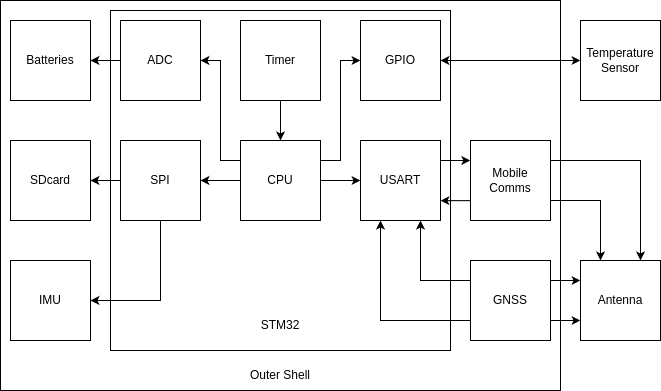
\includegraphics[width=0.9\textwidth]{images/diagrams/block_diagram/block_diagrams_3/blockdiagram_analysis.drawio.png}  % Adjust the width as necessary
    \caption{Block Diagram Initial Draft}
    \label{fig:Block Diagram Initial Draft}        
\end{figure}

The floater draft shows the initial concept of a drifter, as it has the above water 
antenna, a floater to counterbalance the buoy weight, and the temperature sensor. 
According to the blocked diagram.
%corrigir, falta a case no meio e ta mau recortado
\begin{figure}[H]
    \centering
    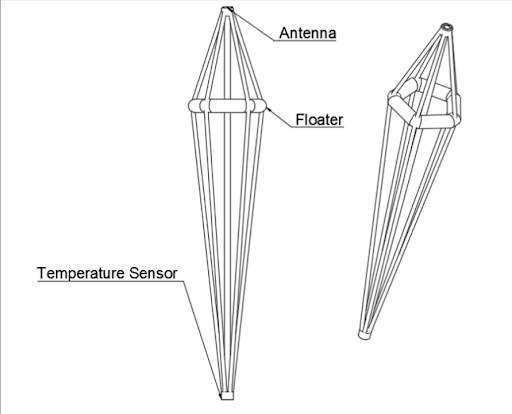
\includegraphics[width=0.7\textwidth]{images/diagrams/shell/unnamed.png}  % Adjust the width as necessary
    \caption{Floater Architecture Initial Draft}
    \label{fig:Floater Architecture Initial Draft}        
\end{figure}

\section{Requirements and Constraints}
\subsection{Requirements}
\begin{itemize}
    \item Search and selection of hardware components.
    \item Software design.
    \item PCB design.
    \item 5S outer shell 3D design.
    \item Actual product realization.
    \item Laboratory tests.
\end{itemize}
\subsection{Constraints}
\begin{itemize}
    \item Limited Team
    \item The project must be presented for evaluation within deadline.
    \item The project has to be validated at the ocean.
    \item The pretended autonomy has to be of a month at minimum.
\end{itemize}

%vila do conde + ou - 10km mar adentro 2g 4g\\
%mapa de alcance na costa\\
%atenção ao clima \\
\section{State of the art}
%%usar fotos do projeto no lab
Nowadays, there are a series of reasons in witch drifters are used. Usually, government 
departments, companies and universities with relations to oceanography, use drifter alike 
to research the local coast for the following reasons.

\begin{itemize}
    \item Border Control
    \item Climate Modeling
    \item Traffic management
    \item Aquaculture management
    \item Public oceanographic research
    \item Marine spatial planning
    \item Defense and security
\end{itemize}

5S drifter aims for \textbf{Climate Modeling}, \textbf{Public oceanographic} or even \textbf{Traffic management} research as this project main objective.
As the data for this project can be used, as stated in the \hyperref[sec:Problem Statement]{Introduction}, to model the environment
in order to better the quality of said topics.
\subsection{Copernicus Example}

The Copernicus Marine Service, component of Copernicus Programme of the 
European Union, has developed the SVP-BRST, a drifter for temperature and depth measurement.
Based on the SSP-B design, the updated version implements a HRSST in addition to the regular 
SST sensor, gathering the position with GNSS and transmitting the data using Iridium.
\begin{figure}[H]
    \centering
    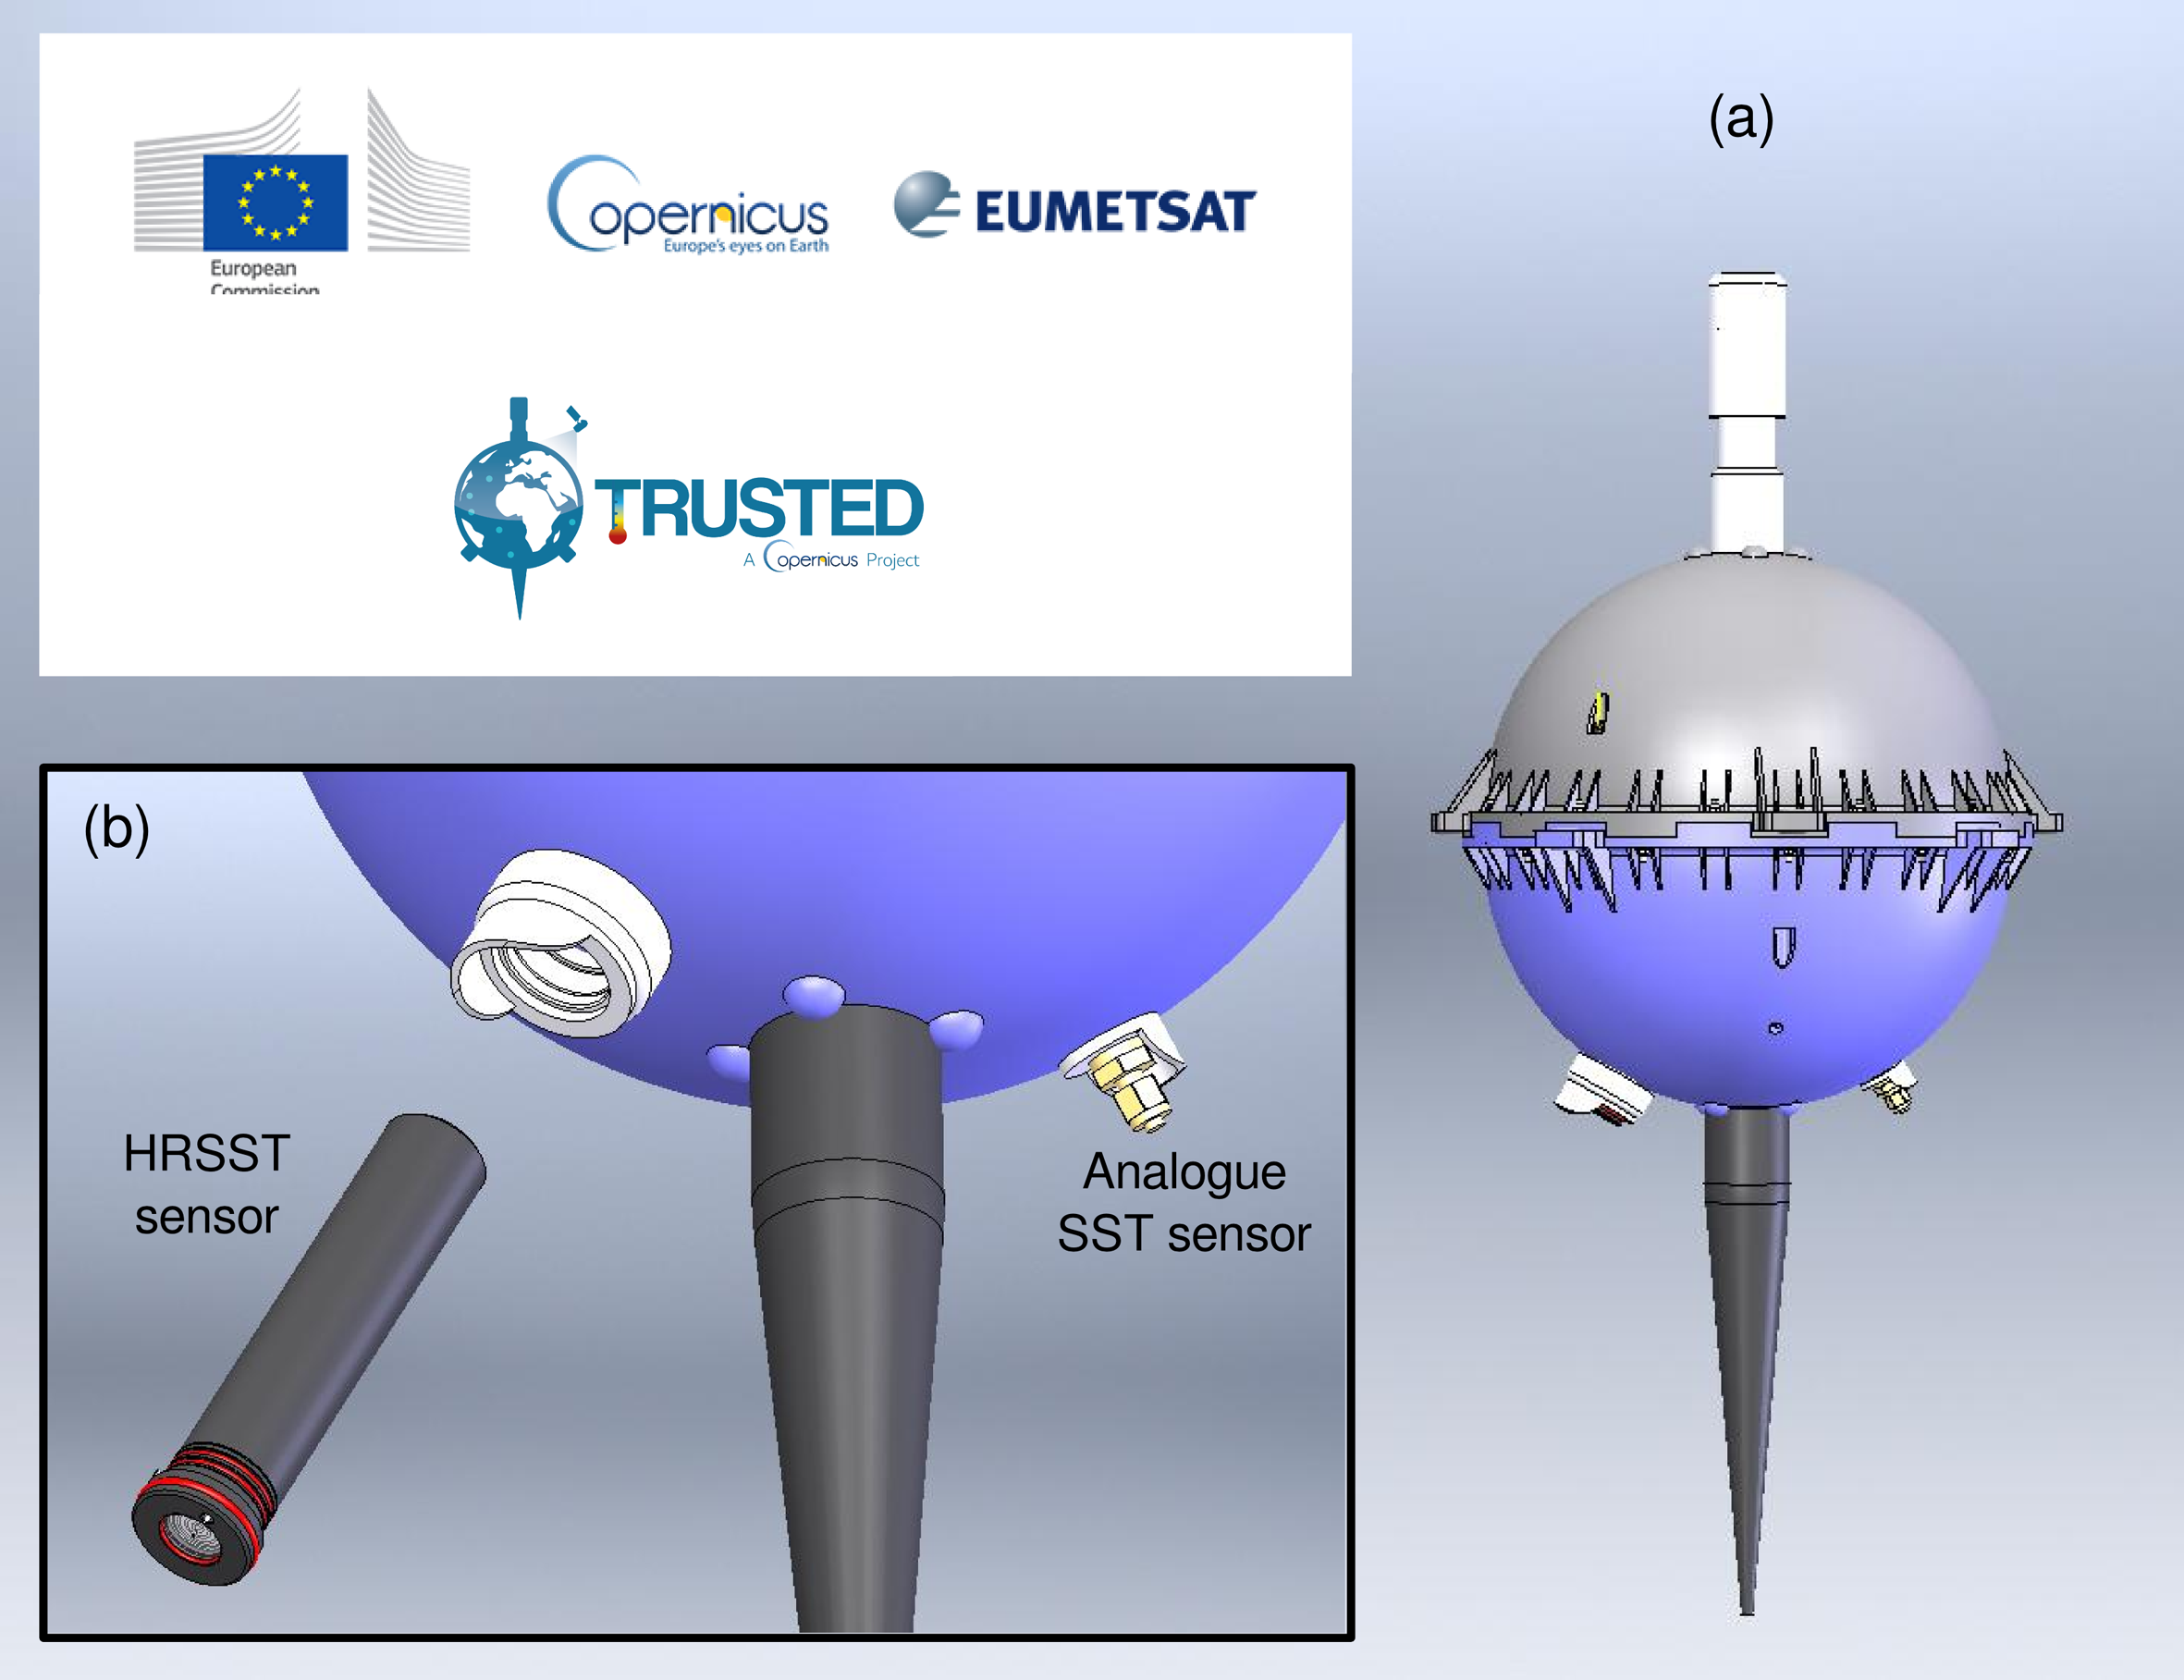
\includegraphics[width=0.55\textwidth]{images/chapter/analysis/svp.png}  % Adjust the width as necessary
    \caption{SVP-BRST Design}
    \label{fig:SVP-BRST Design}        
\end{figure}
The image shows the SVP-BRST model. The (a) image shows the whole model with the antenna the buoyant part ad the weight to point the buoy up.
As for the (b) image, shows the sensor's placement. 

\subsection{CMEMS Examples}
The CMEMS lab at the University of Minho combines expertise 
in microsystems engineering with environmental research to 
develop innovative ocean monitoring technologies. One of 
its key areas involves the design and deployment of autonomous 
drifters to collect real-time data on sea surface conditions 
and currents.

\subsubsection{SONDA}
The project proposes a complementary system for atmospheric
and oceanic monitoring using configurable probes launched by
high-altitude balloons. These probes can measure environmental
parameters from the stratosphere to the deep sea. After 
reaching the seafloor and collecting data (including acoustic 
imaging), the probe resurfaces and transmits the data via 
satellite. It then drifts until its material degrades. The 
system offers a low-cost, high-payload solution with 
limited positional accuracy.

%\begin{wrapfigure}{L}{0.4\textwidth}
%    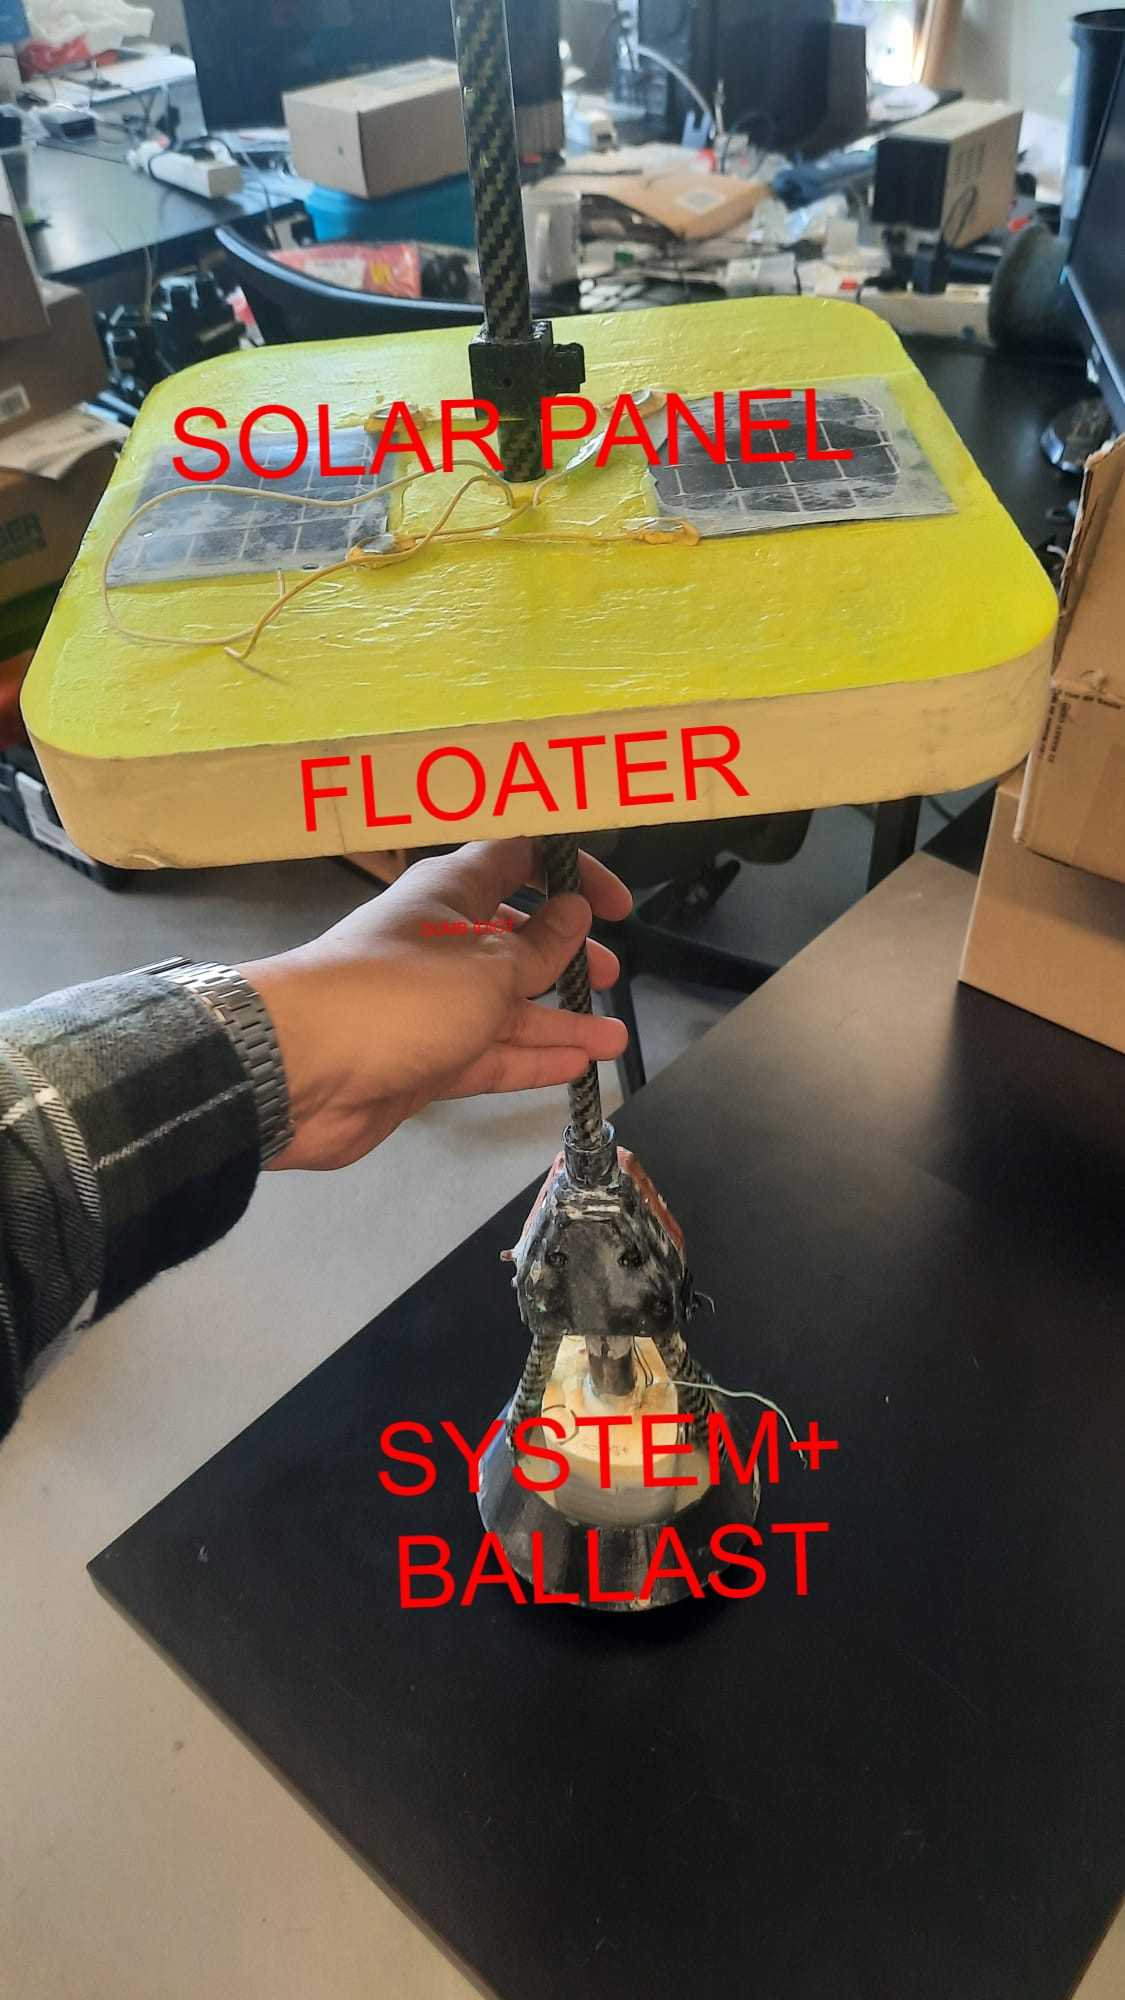
\includegraphics[width=0.25\textwidth]{images/chapter/analysis/sonda_edited.jpg}  % Adjust the width as necessary
%    \caption{SONDA drifter}
%\end{wrapfigure}

\subsubsection{NextSea}
A new approach of monitoring coastal and estuarine relevant variables is presented. MEMS
(Micro Electromechanical Systems), lab-on-chip and microelectronics are used to 
miniaturize and optimize main oceanic sampling. Beyond typical CTD (Conductivity, Temperature
and Depth), other oceanic variables are also monitored. The system also samples type of
phytoplankton and its concentration, pH, currents direction and intensity and turbidity.

\section{System Architecture}

Once studied what the system needs to follow, it is now needed to formulate a solution.
Here it will be used UML diagrams to convey the solution in question, without specific 
implementation details, as this proposal serves to validate and organize the problem 
structure as a formal language.

\subsubsection{Block Diagram}

As previously stated, a block diagram is a formal representation of the system components
and their connection. This one, shows how the peripherals communicate with the microcontroller STM32
as it considers connections with components outside the shell. Initially, as a first analysis
the communication protocol isn't yet defined. However, it will be used to narrow it down.

The diagram shows the SMT32 minimum peripherals: ADC, TIMER, GPIO, I2C / SPI, USART. However,
as it describes the hardware, it doesn't give a good notion on the system software. 

Some points to be considered are:
\begin{itemize}
    \item The temperature sensor communicate using the GPIO, as waterproof sensors, usually, use a driver with specific
    communication protocols.
    \item Mobile Comms is the protocol that will be used to send information to the database. Yet to be chosen. 
    \item GNSS and Mobile Comms for now communicate to the same Antenna, However it probably will use different antennas as different
    protocols require different frequencies to be used.
    \item The communication to the SDcard, uses SPI with STM32 below 64 pins. As it 
    doesn't include SDMMC supporting FatFS.
    \item The batteries power the whole system. Even if not shown.
    \item Depending on the implementation, the timer block will be the Sysclock, as 
    the RTOS may use by default.
\end{itemize}

\begin{figure}[H]
    \centering
    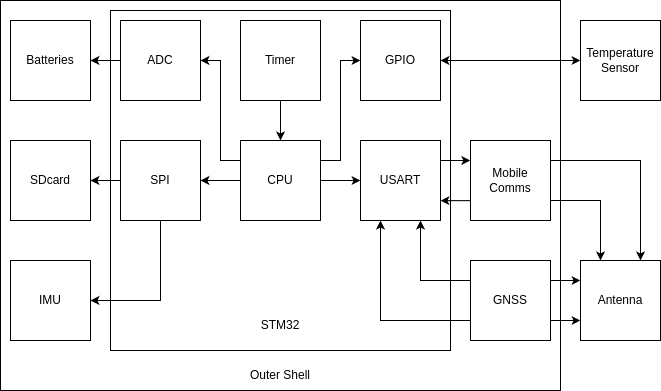
\includegraphics[width=0.9\textwidth]{images/diagrams/block_diagram/block_diagrams_3/blockdiagram_analysis.drawio.png}  % Adjust the width as necessary
    \caption{Block Diagram}
    \label{fig:Block Diagram}        
\end{figure}

\subsubsection{Use Case}

Now, for a software illustration, UML offers a user case, a diagram that exemplifies the system interactions and stimuli.

\begin{figure}[H]
    \centering
    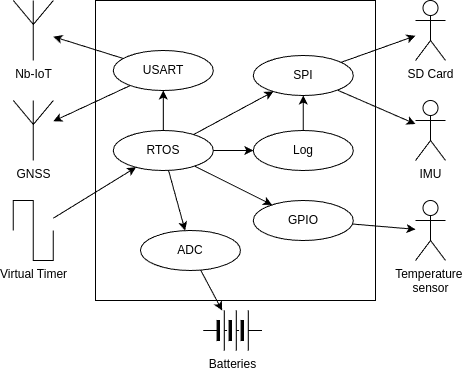
\includegraphics[width=0.6\textwidth]{images/diagrams/use_case/Use Case.drawio.png}  % Adjust the width as necessary
    \caption{Use Case Diagram}
    \label{fig:Use Case Diagram}        
\end{figure}

Now it is introduced to one main component that will be explored further, an RTOS. As it is stimulated by the timer, it will actvate the 
peripherals in a organized form, allowing a fast and efficient use of energy. Other component is the Log, a virtual memory that will store
temporary the information, only storing locally, once per cycle, reducing the SDcard entries.

\subsubsection{Sequence Diagram}

Once the software and hardware are planed, now a time related diagram will show the blocks interactions
as time passes.

First task sequence, a generic "Data Acquisition Task" shows the general behavior of a task focused to manage the sensors.

\begin{figure}[H]
    \centering
    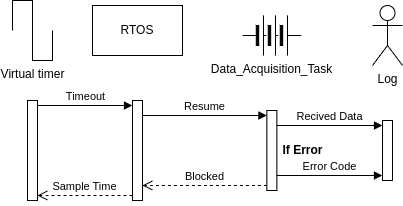
\includegraphics[width=0.7\textwidth]{images/diagrams/sequence_diagram/sequence_diagram_1/Sequence Diagram.drawio.png}  % Adjust the width as necessary
    \caption{Sequence Diagram of Sensor Task}
    \label{fig:Sequence Diagram of Sensor Task}
\end{figure}

Next, the second task sequence, there will be 2 tasks with the behavior to get the GNSS information, store it on log, then call for the Mobile Comms task to send the stored memory to the Database.
On the end, initiating the SDcard storage. 
\begin{figure}[H]
    \centering
    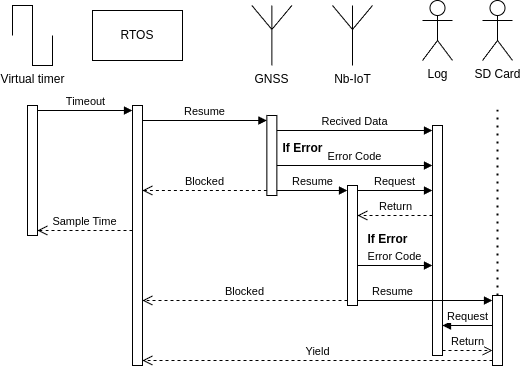
\includegraphics[width=0.7\textwidth]{images/diagrams/sequence_diagram/sequence_diagram_2/Sequence Diagram.drawio.png}  % Adjust the width as necessary
    \caption{Sequence Diagram for Sending and Archive Task}
    \label{fig:Sequence Diagram for Sending and Archive Task}        
\end{figure}

\subsubsection{Threads} 
Once this problem requires a list of tasks to be executed, using a OS will allow
a better project organization and performance with little to no impact in power consumption, 
even helping to manage the low-power mode. However, the implementation will suffer, as the
codification as verification grows, so this topic may become an additional information 
by the end of the project.

As the ST uC offers a variety of RTOS, the implementation will be accessible with good support due to the
CMSIS v2 abstraction layer.

The division in Threads demands a separation in Priority levels, as the OS scheduler takes in consideration 
once both tasks are ready for execution.  

Setting a task priority it must take in vision the resources the task will use, the time it will take to execute said behavior
and the actual importance in matching it time constraints. In order to manage this level of complexity, the RTOS offers a set of
tools for tasks control that will be used for its synchronization and communication.
\begin{itemize}
    \item High Priority Threads \\ 
    Tasks that will handle the outer communication as GNSS and the internet integration will take the higher priority once, as will be handled
    by a peripheral, its execution will be faster, only using the USART interface for AC transmission. 
    \item Normal Priority Threads \\
    The only task here will be the one that has enough importance to be prioritized over the sensors but as the transmission begins it should release the processor
    for the outer communication.
    \item Low Priority Threads \\
    Tasks that only has to measure the sensors having no problem to be removed from the CPU execution
    once their execution is, in their majority, asynchronous.
    
\end{itemize}

%rescrever
\begin{figure}[H]
    \centering
    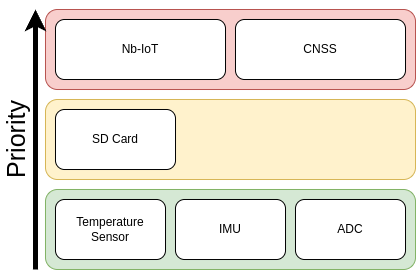
\includegraphics[width=0.7\textwidth]{images/diagrams/threads/thread.drawio.png}  % Adjust the width as necessary
    \caption{Thread Priority Stack}
    \label{fig:Thread Priority Stack}        
\end{figure}

Other important perspective, is to emulate the task behavior with the priorities in action. 
Showing a repetion of X times a group of data acquisition tasks, then ending with the second task sequence.
X yet to be defined as it first depends on the sample time. 
\begin{figure}[H]
    \centering
    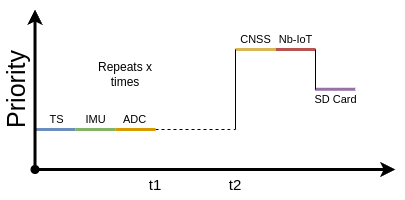
\includegraphics[width=0.7\textwidth]{images/diagrams/threads/graph/threads_graph.drawio.png}  % Adjust the width as necessary
    \caption{Thread Temporal Graph}
    \label{fig:Thread Temporal Graph}        
\end{figure}

Here up to t1 the system executes tasks, storing data, then entering low-power mode until the next sample.
Then, at the end of the last repetition, at t2, stating the second task sequence. Then after the SDcard task behavior ends, and so does the cycle.
\subsubsection{Memory Abstraction (Log)} 

The final diagrams, are a exception to UML diagrams, As it only builds a data structure and a simple interface to interact with it.
Here the idea is to allow memory to be accessible while written by the system, optimizing the RTOS ITCs options.
\begin{figure}[H]
    \centering
    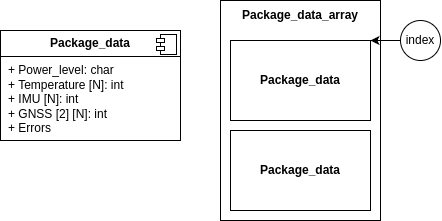
\includegraphics[width=0.7\textwidth]{images/diagrams/data_struct/package_data.drawio.png}  % Adjust the width as necessary
    \caption{Package data structure}
    \label{fig:Package data structure}        
\end{figure}


\begin{figure}[H]
    \centering
    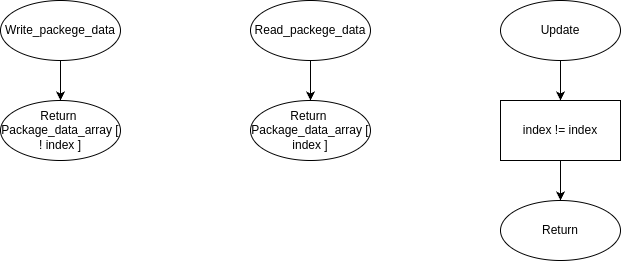
\includegraphics[width=0.75\textwidth]{images/diagrams/data_struct/fluxogram.png}  % Adjust the width as necessary
    \caption{Memory Flowchart}
    \label{fig:Memory Flowchart}        
\end{figure}
